\chapterimage{slike/Nebo.jpg} % Chapter heading image

\chapter{Elektromagnetno valovanje}
Za začetek osvežimo osnove teorije elektromagnetnega polja in elektromagnetnega valovanja. 
Obnovili bomo zapis Maxwellovih enačb, opisali osnovne pojave valovanja (lom, odboj in uklon),
in si ogledali razširjanje svetlobe v anizotropnih snoveh. 

\section{Maxwellove enačbe}
Elektromagnetno polje v praznem prostoru opišemo z dvema vektorskima
poljema, električnim in magnetnim, ki sta v splošnem funkciji prostora
in časa. Vsaki točki v prostoru lahko priredimo \index{Električno polje!jakost}jakost
električnega polja $\mathbf{E}(\mathbf{r},t)$ in \index{Magnetno polje!jakost}jakost
magnetnega polja $\mathbf{H}(\mathbf{r},t)$. Za opis elektromagnetnega
polja v snovi vpeljemo dva dodatna vektorja polja. To sta \index{Električno polje!gostota}gostota
električnega polja $\mathbf{D}(\mathbf{r},t)$ in gostota magnetnega
polja\index{Magnetno polje!gostota} $\mathbf{B}(\mathbf{r},t)$.
Vsa ta polja povezujejo \index{Maxwellove enačbe}Maxwellove enačbe\footnote{
Škotski fizik James Clerk Maxwell, 1831--1879.}
\boxeq{eq:Maxwell1}{
\nabla\times\mathbf{H} & =\frac{\partial\mathbf{D}}{\partial t}+\mathbf{j_e}\\
\nabla\times\mathbf{E} & =-\frac{\partial\mathbf{B}}{\partial t}\label{eq:Maxwell2}\\
\nabla\cdot\mathbf{D} & =\mbox{\ensuremath{\rho}}_{e}\label{eq:Maxwell3}\\
\nabla\cdot\mathbf{B} & =0.\label{eq:Maxwell4}
}\\
Pri zapisu enačb smo upoštevali tudi izvore polj, to je gostoto
električnega toka $\mathbf{j}_e(\mathbf{r},t)$ in gostoto naboja $\rho_{e}(\mathbf{r},t)$. 

Poleg Maxwellovih enačb veljata za vektorski polji zvezi
\begin{align}
\mathbf{D} & =\epsilon_{0}\mathbf{E}+\mathbf{P} \quad \mathrm{in}\\
\mathbf{B} & =\mu_{0}\mathbf{H}+\mu_{0}\mathbf{M},
\end{align}
kjer $\mathbf{P}$ označuje \index{Električna polarizacija}električno
polarizacijo, to je gostoto električnih dipolov, $\mathbf{M}$
pa \index{Magnetizacija}magnetizacijo, to je gostoto magnetnega momenta.
Polarizacija in magnetizacija sta odvisni od zunanjih polj $\mathbf{E}$
in $\mathbf{H}$. V splošnem sta njuni odvisnosti zelo zapleteni,
v izotropnih in linearnih snoveh pa se zvezi poenostavita v 
\beq
\mathbf{P}=\epsilon_{0}\chi_e\mathbf{E} = \epsilon_{0}(\epsilon-1)\mathbf{E} \qquad \textrm{in} 
\qquad
\mathbf{M}=\chi_m \mathbf{H} = (\mu-1)\mathbf{H}
\label{eq:PM}.
\eeq
Vpeljali smo \index{Električna susceptibilnost} električno ($\chi_e$) in 
\index{Magnetna susceptibilnost}magnetno ($\chi_m$) susceptibilnost ter
\index{Dielektričnost}dielektričnost $\epsilon$ in
\index{Magnetna permeabilnost}magnetno permeabilnost $\mu$. Ko združimo gornje
enačbe, lahko zapišemo dve konstitutivni
relaciji
\begin{align}
\mathbf{D} & =\epsilon_{0}\epsilon\mathbf{E}\quad \mathrm{in}\\
\mathbf{B} & =\mu_{0}\mu\mathbf{H}.
\end{align}
V linearnih anizotropnih snoveh moramo namesto skalarnih vrednosti $\varepsilon$
in $\mu$ zapisati tenzorje. 

\subsection*{Robni pogoji}
Navedene Maxwellove enačbe zadoščajo za opis elektromagnetnega polja
v neomejeni snovi, kjer so vse komponente polj zvezne funkcije. Za
obravnavo v omejeni snovi moramo vedeti tudi, kaj se z elektromagnetnim
poljem zgodi na meji dveh sredstev\index{Robni pogoji}. Pri prehodu
iz enega dielektrika v drugega se ohranjata normalni komponenti gostote
električnega in magnetnega polja ter tangentni komponenti jakosti
električnega in magnetnega polja (slika \ref{fig:Robni-pogoji}) 
\boxeq{eq:robni-pogoji}{
D_{1n} &=  D_{2n}\\
B_{1n} &=  B_{2n}\\
E_{1t} &=  E_{2t}\label{eq:robni-pogoji4}\\
H_{1t} &=  H_{2t}.
}
Pri tem smo privzeli, da na meji med dielektrikoma ni površinskih
tokov ali nabojev, sicer bi morali robna pogoja za $D_n$ in $H_t$
ustrezno popraviti. Na meji dielektrika z idealnim prevodnikom (kovino,
zrcalom) so robni pogoji drugačni. Za magnetno polje jih ne moremo
preprosto zapisati, za električno polje pa velja, da mora biti tangentna
komponenta jakosti električnega polja enaka nič. Posledica tega robnega
pogoja je, da se pri pravokotnem vpadu valovanja na zrcalo faza valovanja
spremeni za $\pi$. 

\begin{figure}[h]
\centering
  \def\svgwidth{75truemm} 
  \input{slike/01_robni_pogoji.pdf_tex}
\caption{Na meji med dvema dielektrikoma brez površinskih tokov
in nabojev so tangentna
komponenta jakosti električnega in magnetnega polja ter normalna komponenta
gostote magnetnega in električnega polja zvezne količine.}
\label{fig:Robni-pogoji}
\end{figure}

\section{Valovna enačba in Poyntingov vektor}
Večinoma bomo obravnavali elektromagnetna valovanja v izotropnih, 
homogenih in linearnih snoveh brez zunanjih izvorov in
nosilcev naboja ($\mathbf{j}_e=0$ in $\rho_{e}=0$). 
Iz Maxwellovih enačb (enačbe~\ref{eq:Maxwell1}--\ref{eq:Maxwell4}) izpeljemo valovno 
enačbo\index{Valovna enačba} za jakost električnega ali magnetnega polja 
\boxeq{eq:valovna-skalarna}{
\nabla^{2}\mathbf{E}-\frac{1}{c^{2}}\frac{\partial^{2}\mathbf{E}}{\partial t^{2}} = 0
\quad \mathrm{in} \quad
\nabla^{2}\mathbf{H}-\frac{1}{c^{2}}\frac{\partial^{2}\mathbf{H}}{\partial t^{2}} = 0.
}
Pri tem je hitrost valovanja\index{Hitrost valovanja} v snovi enaka 
\beq
c=\frac{1}{\sqrt{\epsilon\epsilon_{0}\mu\mu_{0}}}=\frac{c_{0}}{n}.
\eeq
Magnetne in dielektrične lastnosti snovi smo pospravili
v lomni količnik\index{Lomni količnik} 
\beq
n=\frac{c_{0}}{c}=\sqrt{\epsilon\mu}.
\eeq
Za izotropno in nemagnetno snov ($\mu=1$) je lomni količnik $n=\sqrt{\epsilon}$.

Vpeljimo še vektor gostote energijskega toka, to je Poyntingov vektor\footnote{Angleški 
fizik John Henry Poynting, 1852--1914.} 
\index{Poyntingov vektor}{$\mathbf{S}$}
\boxeq{eq:Poyntingov-vektor}{
\mathbf{S} = \mathbf{E} \times \mathbf{H}.
}
Kot vidimo, je smer energijskega toka vedno pravokotna na smeri $\mathbf{E}$
in $\mathbf{H}$. Gostoto energijskega toka $j$, to je količino
energije, ki v danem časovnem intervalu preteče skozi dano ploskev
z normalo $\mathbf{\hat{n}}$, izračunamo kot časovno povprečje projekcije
Poyntingovega vektorja \index{Gostota energijskega toka}
\beq
j=\left\langle \mathbf{\mathbf{S}}\cdot\mathbf{\hat{n}}\right\rangle.
\eeq
Gostoti energijskega toka, predvsem gostoti svetlobnega toka, pravimo tudi intenziteta.

\begin{definition}[Poyntingov teorem]
Iz Maxwellovih enačb izpelji kontinuitetno enačbo 
\beq
-\nabla\cdot\mathbf{\mathbf{S}}=\frac{\partial}{\partial t}\left(\frac{1}{2}\epsilon_{0}\mathbf{E}^{2}+
\frac{1}{2}\mu_{0}\mathbf{H}^{2}\right)+\mathbf{E}\cdot\frac{\partial\mathbf{P}}{\partial t}+
\mu_{0}\mathbf{H}\cdot\frac{\partial\mathbf{M}}{\partial t}.
\eeq
Pomagaj si z zvezo $\nabla\cdot(\mathbf{E}\times\mathbf{H})=(\nabla\times\mathbf{E})\cdot\mathbf{H}-
(\nabla\times\mathbf{H})\cdot\mathbf{E}$.
\end{definition}

\index{Poyntingov teorem}Opazimo, da predstavlja Poyntingov teorem
izrek o ohranitvi energije. Prvi in drugi člen na desni strani gornje
enačbe opišeta gostoto energije, shranjene v električnem in magnetnem
polju, medtem ko tretji in četrti člen opišeta energijo,
ki je shranjena v snovi (električnih in magnetnih dipolih). Za valovanje
v homogeni izotropni snovi tako velja
\beq
\nabla\cdot\mathbf{S}=-\frac{\partial w}{\partial t},
\eeq
kjer je $w$\index{Gostota elektromagnetne energije} celotna
gostota energije elektromagnetnega polja. Zapišemo jo kot 
\boxeq{eq:gostota-energije}{
w=\frac{1}{2}\epsilon_{0}\epsilon\mathbf{E}^{2}+\frac{1}{2}\mu_{0}\mu\mathbf{H}^{2}.
}

Valovno enačbo in ohranitvene zakone lahko zapišemo tudi za anizotropne,
nehomogene ali nelinearne snovi. Nekaj teh primerov bomo srečali v nadaljevanju
in jih bomo obravnavali sproti.

\section{Monokromatski elektromagnetni val}

Reševanje valovne enačbe si navadno poenostavimo z vpeljavo kompleksnega
zapisa jakosti električnega in magnetnega polja. Račun si
oglejmo na primeru monokromatskega elektromagnetnega vala. Nastavek
za monokromatski val s krožno frekvenco $\omega$ naj bo\index{Elektromagnetno valovanje}
\beq
\mathbf{E}(\mathbf{r},t)  =\mathfrak{\Re}(\mathbf{E}(\mathbf{r})e^{-i\omega t})\qquad \textrm{in} \qquad
\mathbf{H}(\mathbf{r},t)  =\mathfrak{\Re}(\mathbf{H}(\mathbf{r})e^{-i\omega t}),
\eeq
kjer sta $\mathbf E(\mathbf{r})$ in $\mathbf H(\mathbf{r})$ časovno
neodvisna vektorja jakosti električnega\index{Električno polje!jakost} in 
magnetnega polja\index{Magnetno polje!jakost} s kompleksno
amplitudo. Podobno lahko vpeljemo tudi kompleksne vektorje $\mathbf{P}$,
$\mathbf{M}$, $\mathbf{D}$ in $\mathbf{B},$ ki opisujejo realne količine (polarizacijo,
magnetizacijo, gostoto električnega in gostoto magnetnega polja).
V nadaljevanju bomo večinoma pisali polja v kompleksni obliki, pri
čemer se bomo držali gornje definicije. Zavedati pa se moramo, da
je uporaba kompleksnega zapisa zgolj računski pripomoček, na koncu
je treba rezultate vedno izraziti z realnimi količinami. 

Če vstavimo gornji nastavek za monokromatski val v valovno enačbo
(enačba~\ref{eq:valovna-skalarna}), dobimo \index{Helmholtzeva enačba}Helmholtzevi
enačbi\footnote{Nemški zdravnik in fizik Hermann Ludwig Ferdinand von Helmholtz, 1821--1894.} 
za kompleksna vektorja jakosti električnega in magnetnega polja.
V homogenem in izotropnem sredstvu ju zapišemo kot
\begin{align}
\nabla^{2}\mathbf{E}(\mathbf{r})+k^{2}\mathbf{E}(\mathbf{r}) &=0\label{eq:Helmholtz}\\
\nabla^{2}\mathbf{H}(\mathbf{r})+k^{2}\mathbf{H}(\mathbf{r}) &=0,
\end{align}
kjer je $k=nk_{0}=n\omega/c_{0}$ velikost valovnega vektorja oziroma
valovno število. 

Vpeljimo še kompleksni Poyntingov vektor\index{Poyntingov vektor}
\beq
\mathbf{S}(\mathbf{r})=\frac{1}{2}\mathbf{E}\times\mathbf{H}^{*}.\label{eq:Poyntingov-vektor-c}
\eeq
\begin{definition}
Upoštevajoč izraz za Poyntingov vektor $\mathbf{S}$
(enačba \ref{eq:Poyntingov-vektor}) pokaži, da lahko intenziteto valovanja $j$
(oziroma povprečje projekcije Poyntingovega vektorja)
\index{Gostota energijskega toka} izrazimo
s kompleksnim Poyntingovim vektorjem $\mathbf{S}(\mathbf{r})$:
\beq
\label{eq:jReS}
j=\left\langle \mathbf{\mathbf{S}}\cdot\mathbf{\hat{n}}\right\rangle =
\frac{1}{4}\left(\mathbf{E}\times\mathbf{H}^{*}+\mathbf{E}^{*}\times\mathbf{H}\right)=\Re(\mathbf{S}
(\mathbf{r})).
\eeq
\end{definition}

\section{Ravni val}

Osnovna rešitev valovne enačbe je ravni val\index{Ravni val}. Nastavek, ki predstavlja
ravni val in hkrati reši Helmholtzevo enačbo (enačba~\ref{eq:Helmholtz}), je 
\begin{align}
\mathbf{E}(\mathbf{r},t) & =\mathbf{E}(\mathbf{r})e^{-i\omega t}=
\mathbf{E}_{0}e^{i\mathbf{k}\cdot\mathbf{r}-i \omega t}\quad \mathrm{in}\\
\mathbf{H}(\mathbf{r},t) & =\mathbf{H}(\mathbf{r})e^{-i\omega t}=
\mathbf{H}_{0}e^{i\mathbf{k}\cdot\mathbf{r}-i \omega t},
\end{align}
pri čemer sta vektorja $\mathbf{E}_{0}$ ter $\mathbf{H}_{0}$ od kraja in časa neodvisna. 
Velikost valovnega vektorja $\mathbf{k}$ je $k=nk_{0},$ pri
čemer je $n$ lomni količnik izotropne in homogene snovi. 

Vektorja jakosti električnega in magnetnega polja zadostujeta
Maxwellovim enačbam (enačbe~\ref{eq:Maxwell1}--\ref{eq:Maxwell4}), iz česar sledi,
da sta polji vedno medsebojno pravokotni, 
hkrati pa pravokotni na valovni vektor $\mathbf{k}$. Elektromagnetno valovanje je torej
transverzalno valovanje.

\begin{definition}
\label{naloga-TEM-ortogonalnost}
Pokaži, da za ravni val vedno velja $\mathbf{D} \perp \mathbf{k}$ in 
$\mathbf{B} \perp \mathbf{k}$. Izpelji še pravokotnost polj in valovnega vektorja
v izotropni snovi 
\begin{align}
\mathbf{k}\times\mathbf{H}_{0} & =-\omega\epsilon\epsilon_{0}\mathbf{E}_{0}\label{eq:TEM-pogoj1}\
\quad \mathrm{in}\\
\mathbf{k}\times\mathbf{E}_{0} & =\omega\mu\mu_{0}\mathbf{H}_{0}.\label{eq:TEM-pogoj2}
\end{align}
\end{definition}

Zaradi enolične zveze med električnim in magnetnim poljem zadošča
za opis ravnega vala le eno polje, navadno se odločimo za električno.

Energijski tok je pri ravnem valu v izotropni snovi vedno v smeri valovnega vektorja, pravokotno
na valovne fronte. Iz definicije za gostoto svetlobnega toka (enačbi \ref{eq:jReS} in
\ref{eq:Poyntingov-vektor-c}) ter Maxwellovih enačb (enačbe~\ref{eq:Maxwell1}--\ref{eq:Maxwell4}) 
sledi\index{Gostota energijskega toka}
\beq
j=\Re\left(\frac{1}{4}E_{0}H_{0}^{*}+\frac{1}{4}E_{0}^*H_{0}\right)=
\frac{1}{2}c\epsilon\epsilon_{0}\left|E_{0}\right|^{2}=\frac{1}{2}c_{0}n\epsilon_{0}
\left|E_{0}\right|^{2}.
\eeq
Gostota svetlobnega toka (intenziteta svetlobe) je torej sorazmerna
s kvadratom amplitude jakosti električnega polja. Poglejmo nekaj primerov.
Gostoti toka $j=1~\mathrm{kW/m^{2}}$
(približna gostota svetlobnega toka s Sonca) tako v praznem prostoru ustreza 
jakost električnega polja $E_{0}=868~\mathrm{V/m}$, gostoti $j=1~\mathrm{W/\mu m^{2}}$ 
(intenziteta močno fokusiranega laserskega žarka) pa $E_{0}=27~\mathrm{MV/m}$. 

Zapišimo še povprečno gostoto energije valovanja\index{Gostota elektromagnetne energije}. 
K energiji prispevata tako magnetno kot električno polje. Oba prispevka sta enaka, zato velja
\beq
\left\langle w\right\rangle =\frac{1}{4}\epsilon\epsilon_{0}\left|E_{0}\right|^{2}+
\frac{1}{4}\mu\mu_{0}\left|H_{0}\right|^{2}=\frac{1}{2}\epsilon\epsilon_{0}\left|E_{0}\right|^{2}.
\eeq
Povprečna gostota energije $w$, pomnožena s hitrostjo svetlobe v
snovi, da gostoto energijskega toka $j$ oziroma intenziteto 
svetlobe\index{Gostota energijskega toka}
\boxeq{eq:jcw}{
j=cw.
}
Gornji izraz nazorno kaže, da je intenziteta svetlobe pravzaprav pretok
energije. To si lahko predstavljamo, če vzamemo valj s prečnim presekom
$S$ in dolžino $c\Delta t$. V volumnu $Sc\Delta t$ je potem shranjene $wSc\Delta t$
energije. Energija, ki preteče skozi presek $S$ v času $\Delta t$,
je ravno $cw$. 

Intenziteta ravnega vala je neodvisna od kraja in časa, iz česar sledi,
da je povsod po prostoru enaka. Če bi hoteli izračunati energijo,
ki jo nosi ravni val, bi opazili, da je ta energija neskončna. To
seveda ni mogoče, zato se je vedno treba zavedati, da je ravni val
le idealiziran, a nazoren in praktičen približek elektromagnetnega
vala.

\section{Polarizacija EM valovanja}

Jakost električnega polja elektromagnetnega valovanja je v izotropnem
sredstvu pravokotna na smer valovnega vektorja\footnote{V splošnem je
jakost električnega polja pravokotna na smer Poyntingovega vektorja ($\mathbf{E}\perp\mathbf{S}$) in 
gostota električnega polja pravokotna na smer valovnega vektorja ($\mathbf{D}\perp\mathbf{k}$). 
V anizotropnih sredstvih velja $\mathbf k\nparallel\mathbf S$.}. Vektor $\mathbf{E}$
torej leži v ravnini, pravokotni na smer valovnega vektorja, njegovo
smer pa opiše polarizacija\index{Polarizacija valovanja}. 

V splošnem je ravni val eliptično polariziran. Takrat vektor $\mathbf E$
v ravnini, pravokotni na valovni vektor, oriše elipso. Obe komponenti vektorja 
$\mathbf{E}(\mathbf{r})$ nihata sinusno z enako frekvenco, lahko pa se razlikujeta
v amplitudi in fazi. Kadar je elipsa izrojena v daljico, govorimo o linearno polariziranem valovanju,
kadar pa je krog, govorimo o cirkularno polariziranem valu. Poljubno polarizacijo
lahko vedno zapišemo kot vsoto dveh linearno ali dveh cirkularno polariziranih
valovanj. 

Polarizacijo valovanja lahko zapišemo s kompleksnim \index{Jonesov vektor}Jonesovim 
vektorjem\footnote{Ameriški fizik Robert Clark Jones, 1916--2004.}
$\mathbf{J}$. Za monokromatski ravni val, ki se širi v smeri $z$, je 
\beq
\mathbf{J}=\frac{1}{|E_{0}|}\left[\begin{array}{c}
E_{x}\\
E_{y}
\end{array}\right].
\eeq
Dodali smo normalizacijski faktor $|E_{0}|=\sqrt{|E_{x}|^{2}+|E_{y}|^{2}}$,
da je Jonesov vektor normaliziran in $\mathbf{J}\cdot\mathbf{J}^{*}=1$.
Ravni val, linearno polariziran v smeri $x$, tako zapišemo kot $\mathbf{J}=\left(1,0\right)$,
val, ki je linearno polariziran pod kotom $45^{\circ}$ glede na osi
$x$ in $y$, pa je $\mathbf{J}=\frac{1}{\sqrt{2}}\left(1,1\right)$.
Desno cirkularno polarizirano valovanje zapišemo z vektorjem 
$\mathbf{J}=\frac{1}{\sqrt{2}}\left(1,-i\right)$,
levo cirkularno polarizirano pa z $\mathbf{J}=\frac{1}{\sqrt{2}}\left(1,i\right)$.
Desno polariziran val je torej tisti val, pri katerem se električna
poljska jakost na danem mestu vrti v desno, če gledamo v smeri širjenja
valovanja. Hkrati pa velja, da električna poljska jakost ob danem
času vzdolž smeri širjenja valovanja opiše levosučno vijačnico. 

Zapis z Jonesovim vektorjem je prikladen, saj omogoča preprost izračun
prehoda ravnega vala skozi optične elemente, ki spreminjajo polarizacijo,
a ohranjajo obliko ravnega vala. V splošnem se pri prehodu skozi
sredstvo spremeni kompleksna amplituda $\mathbf{E}_1 = (E_{1x}, E_{1y})$
\begin{align}
E_{2x} & =T_{11}E_{1x}+T_{12}E_{1y}\\
E_{2y} & =T_{21}E_{1x}+T_{22}E_{1y},
\end{align}
pri čemer so komponente $T_{ij}$ odvisne od lastnosti sredstva. Enačbi zapišemo 
v matrični obliki
\beq
\mathbf{E}_{2}=T\cdot\mathbf{E}_{1},
\eeq
kjer sta $\mathbf{E}_{1}$ in $\mathbf{E}_{2}$
vstopni in izstopni val, $T$ pa je \index{Jonesova matrika}Jonesova
matrika. Jonesova matrika za prehod skozi linearni polarizator, ki
polarizira v smeri $x$, je
\beq
T=\left[\begin{array}{cc}
1 & 0\\
0 & 0
\end{array}\right].
\eeq
Oglejmo si še dva zanimiva primera optičnih komponent.
Jonesova matrika za $\lambda/2$ ploščico\index{Ploščica $\lambda/2$},
ki spremeni desno cirkularno polariziran val v levo polariziran in obratno,
je
\beq
T=\left[\begin{array}{cc}
1 & 0\\
0 & -1
\end{array}\right].
\eeq
Jonesova matrika za $\lambda/4$ ploščico\index{Ploščica $\lambda/4$} pa je 
\beq
T=\left[\begin{array}{cc}
1 & 0\\
0 & i
\end{array}\right].
\eeq
Ta optični element linearno polarizirano valovanje oblike $\frac{E_{0}}{\sqrt{2}}(1,1)$
spremeni v levo cirkularno polarizirano valovanje, cirkularno polarizirano
valovanje pa nazaj v linearno. 

\begin{definition}
Pokaži, da je Jonesova matrika za polarizator,
ki prepušča polarizacijo pod kotom $\vartheta$ glede na os $x$, podana z
\beq
T=\left[\begin{array}{cc}
\cos^{2}\vartheta & \sin\vartheta\cos\vartheta\\
\sin\vartheta\cos\vartheta & \sin^{2}\vartheta
\end{array}\right].
\eeq
Namig: matriko $T'$, ki predstavlja polarizator v smeri $x$, zapiši v zavrtenem
koordinatnem sistemu $T=R(\vartheta) \cdot {T'}\cdot R(\vartheta)^\textrm{T}$, 
kjer je $R(\vartheta)$ rotacijska matrika.
\end{definition}

\section{Lom in odboj EM valovanja}

Na ravni meji med dvema izotropnima dielektrikoma se del svetlobe
odbije po odbojnem zakonu, del pa lomi po lomnem zakonu\index{Lomni zakon}
\boxeq{eq:lomni_zakon}{
n_{1}\sin\vartheta_{1}=n_{2}\sin\vartheta_{2}.
}
S kotoma $\vartheta_{1}$in $\vartheta_{2}$ smo označili vpadni in lomni
kot, $n_{1}$in $n_{2}$ pa sta lomna količnika prve in druge snovi.
Poglejmo, kaj se pri lomu in odboju zgodi s polarizacijo valovanja.
Os $x$ naj bo pravokotna na vpadno ravnino (slika~\ref{fig:Lom}). 
Valovanje, polarizirano v tej smeri, je transverzalno električno
(TE) valovanje\index{Polarizacija valovanja!TE}. 
Takrat je električna poljska jakost vzporedna mejni ravnini. 
Kadar leži v mejni ravnini jakost magnetnega polja, govorimo o transverzalnem
magnetnem valovanju (TM)\index{Polarizacija valovanja!TM}.\\

\begin{figure}[h]
\centering \def\svgwidth{120truemm} 
  \input{slike/01_lom.pdf_tex}
\caption{Lom elektromagnetnega valovanja. Levo: transverzalno električno (TE) valovanje. 
Desno: transverzalno magnetno (TM) valovanje. Os $x$ je pravokotna na vpadno ravnino 
in kaže iz lista.}
\label{fig:Lom}
\end{figure}

Jonesovi matriki za prepustnost $t$ in odbojnost $r$ 
na plasti med dvema dielektrikoma zapišemo kot 
\beq
 t=\left[\begin{array}{cc}
t_{x} & 0\\
0 & t_{y}
\end{array}\right]
 \qquad \textrm{in} \qquad 
 r=\left[\begin{array}{cc}
r_{x} & 0\\
0 & r_{y}
\end{array}\right].
\eeq

Potem je 
\begin{align}
E_{2x} & =t_{x}E_{1x} \qquad \qquad E_{3x} =r_{x}E_{1x}\\
E_{2y} & =t_{y}E_{1y} \qquad \qquad E_{3y}=r_{y}E_{1y},
\end{align}
pri čemer smo z $\mathbf{E}_{2}$ označili prepuščeni val, z $\mathbf{E}_{3}$ pa odbitega.
Iz robnih pogojev (enačbe \ref{eq:robni-pogoji}--\ref{eq:robni-pogoji4}) 
izračunamo koeficiente matrik\index{Jonesova matrika}
$r$ in $t$ s \index{Fresnelove enačbe}Fresnelovimi 
enačbami\footnote{Francoski fizik Augustin-Jean Fresnel, 1788--1827.}:
\beq
r_{x}=\frac{n_{1}\cos\vartheta_{1}-n_{2}\cos\vartheta_{2}}{n_{1}\cos\vartheta_{1}+n_{2}\cos\vartheta_{2}},
\qquad t_{x}=1+r_{x}=\frac{2n_{1}\cos\vartheta_{1}}{n_{1}\cos\vartheta_{1}+n_{2}\cos\vartheta_{2}}
\eeq
in
\beq
r_{y}=\frac{n_{2}\cos\vartheta_{1}-n_{1}\cos\vartheta_{2}}{n_{1}\cos\vartheta_{2}+n_{2}\cos\vartheta_{1}},
\qquad t_{y}=(1+r_{y})\frac{\cos\vartheta_{1}}{\cos\vartheta_{2}}=\frac{2n_{1}\cos\vartheta_{1}}
{n_{1}\cos\vartheta_{2}+n_{2}\cos\vartheta_{1}}.
\eeq

V splošnem sta odbojnost $r$ in prepustnost $t$ kompleksni
količini, saj iz lomnega zakona sledi, da je $\cos\vartheta_{2}=
\sqrt{1-\left(n_{1}/n_{2}\right)^{2}\sin^{2}\vartheta_{1}}$
lahko kompleksen. Velikost števila $\left|r\right|$ tako predstavlja
odbojnost, argument $\arg\{r\}$ pa spremembo faze
pri odboju.

Prepustnost $r$ in odbojnost $t$ povesta, kako se spremeni kompleksna
amplituda jakosti električnega polja. Razmerje med intenziteto odbite
in vpadne svetlobe $\mathcal{R}$ oziroma razmerje med intenziteto prepuščene in vpadne svetlobe
$\mathcal{T}$ izračunamo kot 
\beq
\mathcal{R}=\left|r\right|^{2}
\eeq
in
\beq
\mathcal{T}=1-\mathcal{R}.
\eeq
Slednja enačba sledi iz ohranitve energije. V splošnem $\mathcal{T}$
ni enak $\left|t\right|^{2},$ saj energijski tok potuje po različnih
snoveh in v različnih smereh. Velja zveza
\beq
\mathcal{T}=\frac{n_{2}\cos\vartheta_{2}}{n_{1}\cos\vartheta_{1}}\left|t\right|^{2}.
\eeq

Zanimiva je odvisnost odbojnosti od vpadnega kota. Izkaže se, da pri nekem kotu, 
imenujemo ga \index{Brewsterjev kot}Brewsterjev kot\footnote{Škotski fizik in znanstvenik Sir David Brewster, 1781--1868.}, 
odbojnost za TM polarizacijo enaka nič in vsa vpadla
svetloba je prepuščena. Brewsterjeva
okna (steklene ploščice, postavljene pod Brewsterjevim kotom) uporabljamo
v resonatorjih laserjev za povečanje izgub TE in zmanjšanje izgub
TM polariziranega valovanja.

\begin{definition}[Brewsterjev kot]
Pokaži, da za TM val obstoja vpadni kot
\beq
\vartheta_{B}=\arctan\left(\frac{n_2}{n_1}\right),
\eeq
pri katerem je odbojnost enaka nič in prepustnost enaka $\mathcal{T}=$1.
\end{definition}

\begin{remark}
Pri prehodu skozi optične elemente se --
razen TM polariziranega valovanja pri Brewsterjevem 
kotu -- vedno nekaj
svetlobe odbije. Da zmanjšamo te izgube, optične elemente navadno
prekrijemo z antirefleksno plastjo, to je nanosom ene ali več primerno
izbranih debelin plasti dielektrikov z ustreznimi lomnimi količniki.
Zaradi destruktivne interference se količina odbite svetlobe z izbrano
valovno dolžino občutno zmanjša. Ker imamo v fiziki laserjev opraviti
s koherentnimi izvori s točno določeno valovno dolžino, za zmanjšanje
izgub, na primer v resonatorju laserja, vedno uporabljamo optične
elemente (leče, kristale, akusto-optične modulatorje ... ) z ustrezno
antirefleksno plastjo.
\end{remark}

\section{Uklon svetlobe}

Ko svetloba vpade na oviro, za oviro nastane senca. Nastala senca ni ostra, ampak
ima zaradi uklona zabrisane robove. Obravnave 
uklona svetlobe na odprtinah (zaslonkah) se najenostavneje lotimo z uporabo
skalarnega približka teorije elektromagnetnega polja. To pomeni, da vpliv 
polarizacije zanemarimo. Vpliv polarizacije je pomemben zgolj pri zelo majhnih odprtinah, 
torej kadar je $\lambda\sim a$, kjer je $a$ velikost
odprtine. Treba pa je povedati, da so tudi v tem primeru uklonske slike za 
različne polarizacije podobne, razlikujejo pa se po intenziteti prepuščene svetlobe.

\begin{remark}{{\bf Žičnati polarizatorji}}\\ \\
Primer, kjer skalarni približek ne da pravih rezultatov, je uklon na mrežici, narejeni 
iz zelo tankih prevodnik žic s periodo mrežice $d\ll \lambda$. Takšna mrežica 
deluje kot polarizator za valovanje s polarizacijo, ki je pravokotno na žice (TE polarizacija). 
Elektromagnetni val s TM polarizacijo pri prečkanju inducira tok v žicah, medtem
ko je za TE polarizacijo inducirani tok bistveno manjši, saj je smer toka omejena
vzdolž žice. Posledično je prepustnost za TE val velika, medtem ko se TM val delno
absorbira in odbije. Takšni polarizatorji se večinoma uporabljajo v mikrovalovni tehniki, 
vendar se v zadnjih letih z razvojem in izboljšavo litografskih postopkov
vse pogosteje uporabljajo tudi v bližnjem infrardečem področju svetlobe.
\end{remark}

Pri dimenzijah odprtin $a>\lambda$ torej lahko uporabimo skalarno teorijo, zato zapišemo
valovno enačbo (enačba~\ref{eq:valovna-skalarna}) v skalarni obliki
\beq
\nabla^2 E - \frac{1}{c^2}\frac{\partial^2 E}{\partial t^2} = 0.
\label{eq:skalarna-valovna-enačba}
\eeq
Zapisana valovna enačba velja za vse komponente električne $E$ in tudi 
magnetne poljske jakosti $H$. Časovna odvisnost polja $E$ je harmonična funkcija in 
je sorazmerna z $e^{-i \omega t}$. Z uporabo Greenovega teorema lahko 
jakost polja $E_P$ v točki $P$ izrazimo s poljem na poljubni ploskvi, ki obkroža točko $P$. 
Zvezo opisuje Kirchhoffov integral\footnote{Nemški fizik Gustav Kirchhoff, 1824--1887.} 
\index{Kirchhoffov integral}
\beq
E_P = -\frac{1}{4\pi}\oint \left(E\,\mathbf{n}\cdot \nabla \frac{e^{ikr}}{r}-
\frac{e^{ikr}}{r}\mathbf{n}\cdot \nabla E \right) dS,
\label{eq:Kirchhoffov-integral}
\eeq
kjer je $\mathbf{n}$ normala na ploskev, po kateri teče integral, $r$ pa je oddaljenost od točke P
do ploskve $dS$ (slika \ref{fig:UklonFK}). Kirchhoffov integral velja splošno za katerokoli harmonično 
funkcijo, ki reši valovno enačbo (enačba~\ref{eq:skalarna-valovna-enačba}), ne samo $E$ in torej
ni vezan na obravnavo uklona svetlobe. 

Kot prvi primer vzemimo točkast izvor v točki $S$. Svetloba iz njega vpada na zaslon, 
v katerem je odprtina poljubne oblike. Izračunajmo skalarno polje v točki $P$ na drugi 
strani zaslona. Vpadno svetlobo zapišemo kot
\beq
\label{eq:polje-krogelni-val}
E = A \frac{e^{ikr'}}{r'},
\eeq
kjer je $r'$ razdalja od izvora do točke na zaslonu, A pa zaradi ohranitve energije konstanta.

\begin{figure}[h]
\centering \def\svgwidth{75truemm} 
  \input{01_uklonFK.pdf_tex}
\caption{Integracijska ploskev v Kirchhoffovem integralu zajema odprtino in objema točko $P$.}
\label{fig:UklonFK}
\end{figure}


Integracijska ploskev je lahko poljubna sklenjena ploskev, ki objema točko $P$. Izberemo tako, ki
zajema odprtino na zaslonu, poleg tega pa naredimo še dva približka:\\
\begin{enumerate}
\item Jakost polja $E$ in njen gradient doprineseta k integralu le na odprtini, na preostanku ploskve
pa sta njuna prispevka zanemarljivo majhna.\\
\item Vrednost $E$ in njen gradient sta na odprtini takšna, kot da zaslona ne bi bilo.\\
\end{enumerate}
Zgornja približka sta precej groba, vendar se izkaže, da v splošnem kljub temu
dobimo dobro ujemanje z eksperimentalno določeno uklonsko sliko, s čimer 
upravičimo njuno uporabo pri izračunu uklonske slike.

Kirchhoffov integral za primer točkastega izvora svetlobe se potem zapiše kot
\beq
E_P = -\frac{ik A e^{-i\omega t}}{4\pi}\int\frac{e^{ik(r+r')}}{rr'}\left[\cos(\mathbf{n},
\mathbf{r})-\cos(\mathbf{n},\mathbf{r'})\right] dS.
\label{eq:Fresnel-Kirchoffov-integral}
\eeq
V literaturi ga pogosto imenujejo Fresnel-Kirchhoffov uklonski integral\footnote{Francoski fizik
Augustin-Jean Fresnel, 1788--1827.}\index{Fresnel-Kirchhoffov uklon}.
\begin{definition}
\label{naloga-Fresnel-Kirchhoff-uklon}
Uporabi Kirchhoffov integral in pokaži, da je za primer krožnega vpadnega vala
(enačba~\ref{eq:polje-krogelni-val}) polje v točki $P$, ki je od odprtine oddaljena 
$r \gg \lambda$, zapišemo z enačbo~(\ref{eq:Fresnel-Kirchoffov-integral}).
\end{definition}

Oglejmo si poseben primer, ko leži točkast izvor svetlobe na osi okrogle odprtine. Razdalja
$r'$ je potem konstantna in polje v točki $P$ izračunamo kot 
\beq
\label{eq:Fresnelov-uklon}
E_P =  -\frac{ik}{4\pi} \int E_S\frac{ e^{ikr-i\omega t}}{r}\left[\cos(\mathbf{n},\mathbf{r})+1\right] dS,
\eeq
pri čemer $E_S$ predstavlja kompleksno amplitudo vpadnega polja v odprtini
\beq
E_S = A \frac{e^{ikr'}}{r'}.
\eeq 
Zgornja oblika Fresnel-Kirchhoffovega integrala ni pravzaprav nič drugega kot 
matematičen zapis \index{Huygensovo načelo}Huygensovega 
načela\footnote{Nizozemski znanstvenik Christiaan Huygens, 1629--1695.}. 
Spomnimo se, da Huygensovo načelo pravi, da lahko vsako točko valovne fronte obravnavamo 
kot izvor novega krogelnega vala. Točno to je zapisano tudi v gornjem integralu. Vpadni val
$E_S$ v vsakem od elementov $dS$ odprtine vzbudi krogelno valovanje s
kompleksno amplitudo
\beq
E = A_0 \frac{e^{ikr}}{r},
\eeq 
polje v izbrani točki $P$ pa je vsota prispevkov posameznih krogelnih valovanj.

Za razliko od osnovnega Huygensov načela, v enačbi (\ref{eq:Fresnel-Kirchoffov-integral})
nastopa še faktor $\left[\cos(\mathbf{n},\mathbf{r})-1\right]$, ki poskrbi, da ni valovanja 
v smeri nazaj proti izvoru. Tudi faktor $-i$ manjka v osnovnem Huygensovem načelu,
pomeni pa, da je uklonjeno valovanje fazno zakasnjeno za $\pi/2$ glede na osnovno
valovanje $E_S$.

Uporabna razširitev Fresnel-Kirchhoffovega uklona je z uporabo prepustnostne funkcije odprtine $T$.
Z njo v splošnem popišemo amplitudne in fazne spremembe, do katerih lahko pride na raznih 
odprtinah, lečah, uklonskih mrežicah ... Razširjen uklonski integral zapišemo kot
\beq
\label{eq:Fresnelov-uklon2}
E_P =  -\frac{ik}{4\pi} \int T(r) E_S(r) \frac{ e^{ikr-i\omega t}}{r}
\left[\cos(\mathbf{n},\mathbf{r})+1\right] dS,
\eeq
pri čemer smo upoštevali tudi splošno obliko vpadnega vala $E_S(r)$.

\subsection*{Fraunhoferjev in Fresnelov približek}
\label{FFuklon}
Izračun Fresnel-Kirchhoffovega integrala je v splošnem zelo zapleten, zato se 
pogosto poslužimo dveh približkov: Fraunhoferjevega\footnote{Nemški fizik 
Joseph von Fraunhofer, 1787--1826.} in Fresnelovega\index{Fresnelov uklon}. 
Fraunhoferjeva uklonska slika\index{Fraunhoferjev uklon} velja za daljno polje, kadar lahko 
vpadni in uklonjeni val zapišemo kot ravna valova. Bolj zapleteno Fresnelovo uklonsko sliko pa moramo
uporabiti, kadar obravnavamo primer bližnjega polja. 
\begin{figure}[h]
\centering \def\svgwidth{100truemm} 
  \input{slike/01_uklonFF.pdf_tex}
\caption{Različna približka za obravnavo uklona na odprtini. Fraunhoferjev (levo) velja za daljno polje,
Fresnelov (desno) pa za bližnje.}
\label{fig:UklonFF}
\end{figure}

Mejo med daljnim in bližnjim poljem kvalitativno določa Fresnelovo število\index{Fresnelovo število}
\beq
F= \frac{a^2}{L\lambda},
\eeq 
kjer je $a$ karakteristična dimenzija odprtine, $L$ tipična oddaljenost od odprtine ter
$\lambda$ valovna dolžina. V grobem velja, da za oddaljenosti $L$ od odprtine, za
katere velja $F<1$, polje obravnavamo kot daljno polje, medtem ko $F>1$ pove, da 
moramo uklon obravnavati v Fresnelovem približki ali celo v polni obliki. 



Zapišimo uklonske integrale za oba približka. Izhajajmo iz Fresnel-Kirchhofovega integrala
(enačba~\label{eq:Fresnelov-uklon}) in zapišimo razdaljo $r$ s koordinatama na zaslonu $x', y'$ ter
lego točke $P$ s koordinatami $x,y,z$ (slika \ref{fig:Uklon-koordinate})

\begin{figure}
\centering \def\svgwidth{100truemm} 
  \input{01_uklon_koordinate.pdf_tex}
\caption{K izračunu Fraunhhoferjeve in Fresnelove uklonske slike}
\label{fig:Uklon-koordinate}
\end{figure}

\beq
r = \sqrt{(x-x')^2+(y-y')^2 + z^2}.
\eeq
Privzemimo, da je $z$ razmeroma velik v primerjavi s prečnima razlikama in lahko $r$ razvijemo
\beq
r \approx z + \frac{(x-x')^2}{2z} +\frac{(y-y')^2}{2z}.
\eeq
V Fraunhoferjevem približku zadošča uporaba le linearnih členov v gornjem izrazu in za Fraunhoferjev
uklonski integral dobimo
\beq
\label{eq:FraunhoferApprox}
E_P =  -\frac{i}{z\lambda} \int \int E_S e^{-ik (xx'+yy')/z} dx' dy',
\eeq
kar ni nič drugega kot Fouriereva transformacija polja $E_S$.

V Fresnelovem približku upoštevamo tudi kvadratne člene v razvoju in dobimo
\beq
\label{eq:FresnelApprox}
E_P =  -\frac{i}{z\lambda} \int \int E_S e^{-ik ((x-x')^2+(y-y')^2)/2z} dx' dy'.
\eeq

\begin{definition}
\label{naloga-Fresnel-Kirchhoff-uklon}
Pokaži, da je v Fraunhoferjevi uklonski sliki uklon na okrogli odprtini s premerom $a$ podan z
\beq
E_P = E_0\frac{J_1(\pi a \rho/ \lambda z)}{\pi a \rho/ \lambda z},
\eeq
kjer je $\rho = \sqrt{x^2+y^2}$.
\end{definition}

\section{EM valovanje v anizotropnih snoveh}

Do zdaj smo obravnavali elektromagnetno valovanje
v izotropnih snoveh, v katerih je dielektričnost skalar in hitrost širjenja
valovanja neodvisna od njegove smeri. V splošnem so snovi anizotropne,
dielektričnost\index{Dielektričnost} je tenzor, hitrost potovanja svetlobe skozi snov pa
je odvisna od smeri razširjanja in od polarizacije valovanja. 

Gostoto električnega polja v anizotropni snovi zapišemo kot 
\beq
\mathbf{D}=\epsilon_{0}\underline{\epsilon} \cdot\mathbf{E} = 
\epsilon_{0}
\left[\begin{array}{ccc}
\epsilon_{11} & \epsilon_{12}& \epsilon_{13}\\
\epsilon_{21} & \epsilon_{22}& \epsilon_{23}\\
\epsilon_{31} & \epsilon_{32}& \epsilon_{33}\\
\end{array}\right]\mathbf{E},
\label{eq:gostota-elektricnega-polja-tenzor}
\eeq
kjer je $\epsilon_{ij}$ tenzor drugega reda in ima v splošnem devet komponent.
V dielektričnih snoveh, v katerih ne pride do optične aktivnosti ali absorpcije, je tenzor
realen in simetričen $\epsilon_{ij}=\epsilon_{ji}^*$. Tak tenzor lahko vedno
diagonaliziramo, torej poiščemo koordinatni sistem, v katerem je tenzor $\underline{\epsilon}$
diagonalen. V takem koordinatnem sistemu velja 
\beq
\mathbf{D} = \epsilon_{0}
\left[\begin{array}{ccc}
\epsilon_{1} & 0& 0\\
0 & \epsilon_{2}& 0\\
0 & 0& \epsilon_{3}\\
\end{array}\right]\mathbf{E}
\eeq
in 
\beq
D_{1}=\epsilon_{0}\epsilon_{1}E_{1},\quad D_{2}=\epsilon_{0}\epsilon_{2}E_{2},\quad D_{3}=
\epsilon_{0}\epsilon_{3}E_{3}.\label{eq:gostota-elektricnega-polja-lastni}
\eeq
Glavne osi sistema določajo smeri, vzdolž katerih sta jakost
in gostota električnega polja vzporedni, lastne vrednosti 
pa ustrezajo trem lomnim količnikom\index{Lomni količnik} $\epsilon_{i}=\sqrt{n_{i}}$. Kristale,
za katere so vse tri vrednosti $n_i$ različne, imenujemo optično dvoosni kristali\index{Dvoosni
kristali}, medtem ko sta v optično enoosnih\index{Enoosni kristali} 
kristalih dve lastni vrednosti enaki $n_{1}=n_{2}$. 
Če so enake vse tri vrednosti, je snov izotropna.

\subsection*{Optična indikatrisa}
Poglejmo, kako se po anizotropnih snoveh širi valovanje v odvisnosti
od njegove smeri in polarizacije. Preprost primer je valovanje, ki se širi vzdolž lastne
osi $z$, polarizirano pa je vzdolž lastne osi $x$. Pri prehodu
skozi kristal se polarizacija valovanja ohrani, lomni količnik za
tak val pa je $n_{1}$. Podobno velja za val, polariziran v smeri
$y$, za katerega je lomni količnik enak $n_{2}$. Če se valovanje širi vzdolž lastne
osi $z$, vendar njegova polarizacija ne sovpada z lastnima osema
$x$ ali $y$, dobimo po prehodu skozi kristal iz vpadnega linearno polariziranega valovanja
v splošnem eliptično valovanje. Lastni komponenti namreč potujeta z različnima
hitrostma, zato pride med njima do faznega zamika.\\
\begin{figure}[h]
\centering
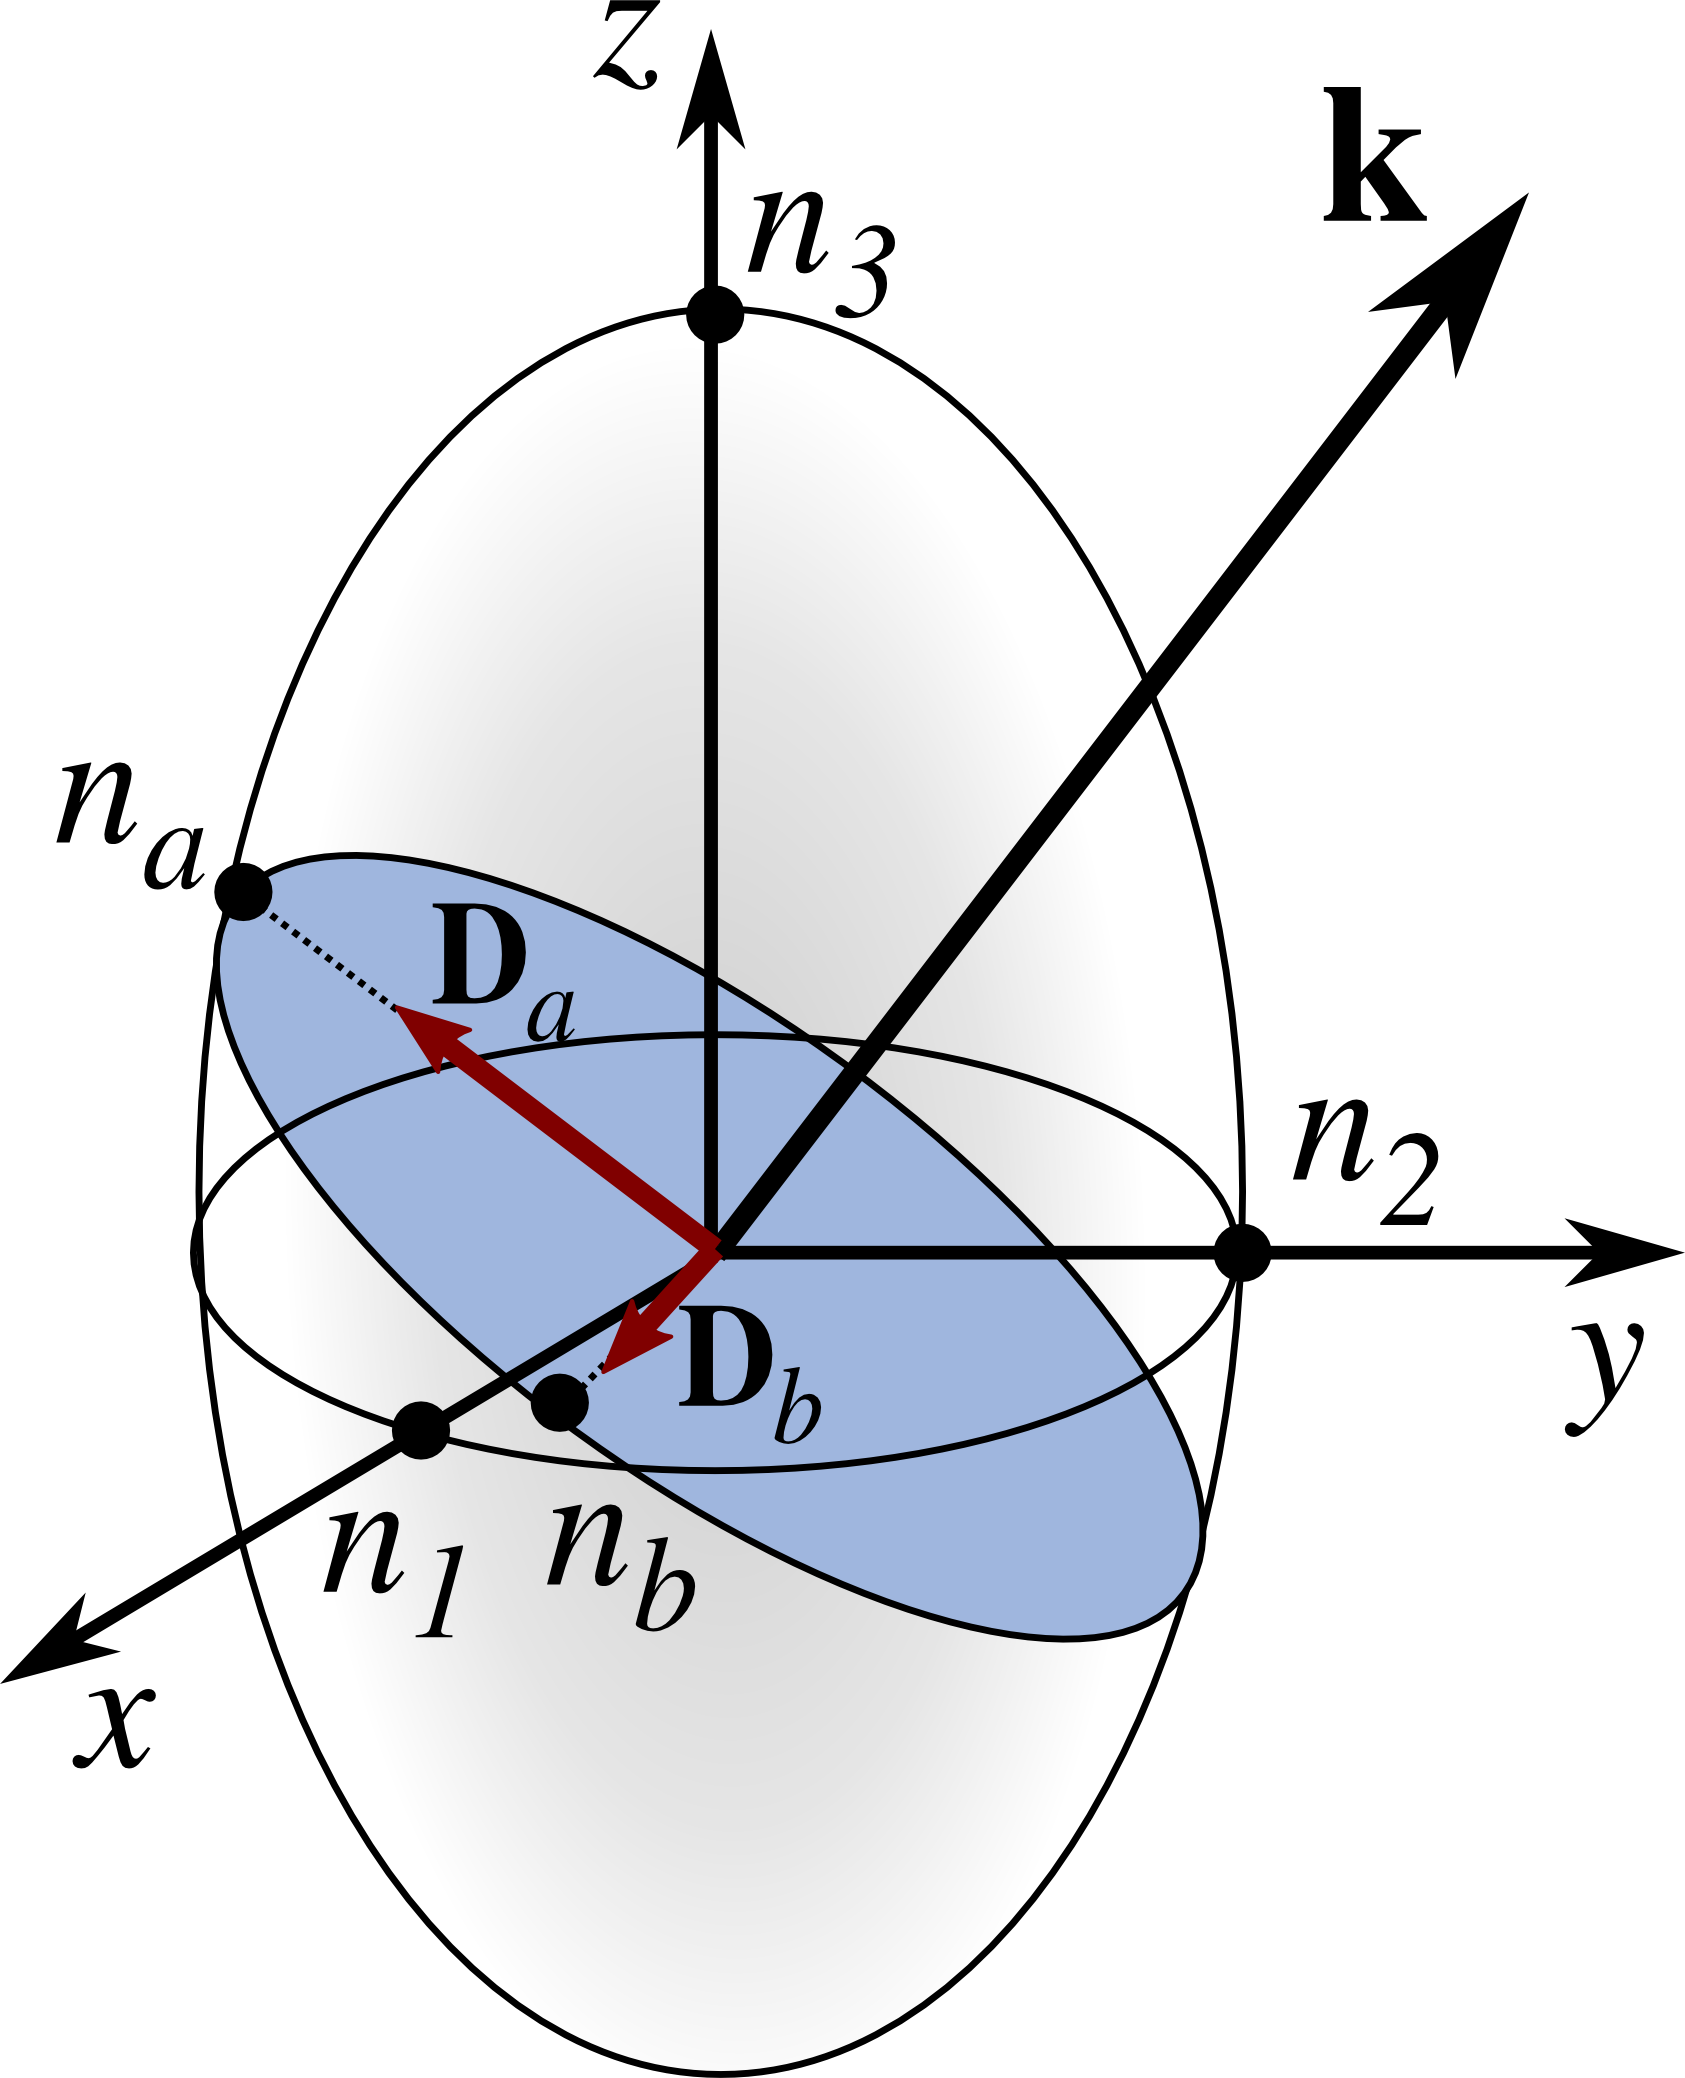
\includegraphics[width=4truecm]{slike/01_indikatrisa.png}
\caption{\label{fig:Indikatrisa}Optična indikatrisa oziroma elipsoid lomnega količnika. Glavne osi
elipsoida sovpadajo z glavnimi osmi tenzorja $\varepsilon$, polosi elipsoida pa so enake
lomnim količnikom $n_i$. V primeru optično enoosnega kristala je indikatrisa  
rotacijski elipsoid, v primeru izotropne snovi pa je optična indikatrisa krogla. }
\end{figure}


Za poljubno smer širjenja valovanja ter poljubno polarizacijo je račun
bolj zapleten in je treba lomne količnike še izračunati. Pri tem si pomagamo 
z grafično upodobitvijo, s tako imenovano 
\index{Optična indikatrisa}optično indikatriso (elipsoidom lomnega
količnika). Optična indikatrisa je elipsoid, podan z enačbo
\beq
\frac{x^{2}}{n_{1}^{2}}+\frac{y^{2}}{n_{2}^{2}}+\frac{z^{2}}{n_{3}^{2}}=1.
\eeq
Glavne osi elipsoida sovpadajo z glavnimi osmi tenzorja $\epsilon$, 
polosi elipsoida pa so $n_{1}$, $n_{2}$ in $n_{3}$. 
Za val, ki se širi z valovnim vektorjem $\mathbf{k}$, skozi izhodišče
narišemo ravnino, pravokotno na smer valovnega vektorja (slika \ref{fig:Indikatrisa}).
Presečišče ravnine in elipsoida je elipsa, katere glavni osi podata
vrednosti lomnih količnikov $n_{a}$ in $n_{b}$ za obe lastni polarizaciji,
njuni smeri pa predstavljata lastni smeri gostote električnega polja. Ker
sta to lastni osi, smer jakosti električnega polja izračunamo z
enačbo (\ref{eq:gostota-elektricnega-polja-lastni}).

\subsection*{Optično enoosni kristali}
V optično enoosnih kristalih sta dve lastni vrednosti enaki in indikatrisa je rotacijski 
elipsoid. Po dogovoru izberemo lastne vrednosti tako, da velja $n_{1}=n_{2}\neq n_{3}$. 
Za valovanje, ki se razširja v smeri $z$, sta lomna količnika za obe polarizaciji 
enaka in os $z$ imenujemo \index{Optična os}optična os. Hitrost valovanja, ki
se širi vzdolž optične osi, je torej neodvisna od njegove polarizacije.
Navadno vpeljemo tudi nove oznake: $n_{1}=n_{2}=n_{o}$, ki označuje redni (\textit{ordinary})
lomni količnik, $n_{3}=n_{e}$ pa izredni (\textit{extraordinary}) lomni količnik. 


Zaradi simetrije je pri izračunu lomnega količnika pomemben le kot 
$\vartheta$ med valovnim vektorjem $\mathbf{k}$ in optično osjo $z$. Dvema 
lastnima polarizacijama pripadata dva različna lomna količnika. 
Za lažjo predstavo oba lomna količnika skiciramo v odvisnosti
od kota $\vartheta$ (slika~\ref{fig:Elipsa}). Lomni količnik za žarek, ki
je polariziran pravokotno na vpadno ravnino, je neodvisen od $\vartheta$, zato narišemo krožnico.
Takemu žarku pravimo \index{Redni žarek}redni žarek. 
Žarek, ki je polariziran v vpadni ravnini, je tako imenovan izredni žarek. Pripadajoč
lomni količnik je odvisen od kota $\vartheta$ in ga izračunamo iz sledeče enačbe elipse
s polosema $n_o$ in $n_e$: 
\beq
\frac{1}{n^{2}(\vartheta)}=\frac{\cos^{2}\vartheta}{n_{o}^{2}}+\frac{\sin^{2}\vartheta}{n_{e}^{2}}.
\label{eq:izreden}
\eeq
Opazimo, da se krožnica in elipsa dotikata ravno na osi $z$. Takrat se 
valovanje širi vzdolž optične osi in lomna količnika sta za obe polarizaciji enaka $n_o$. 

\begin{figure}[h]
\centering
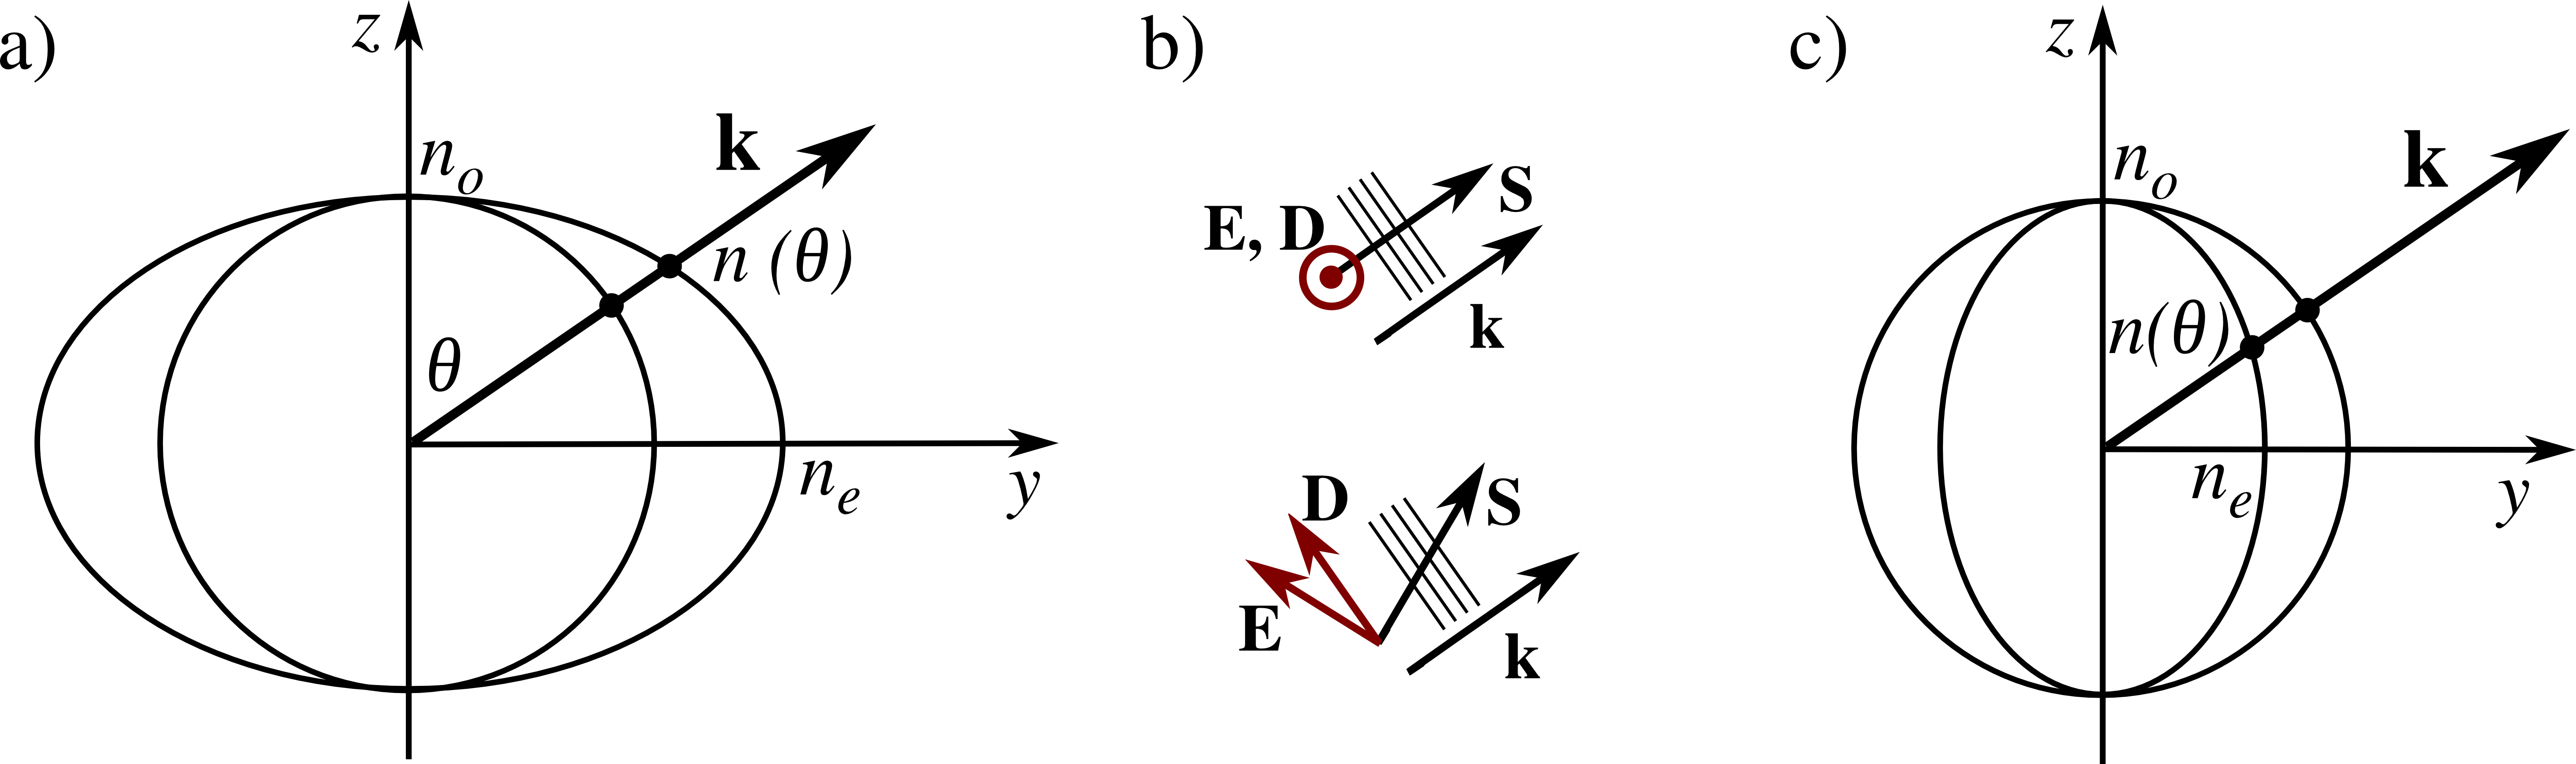
\includegraphics[width=12truecm]{slike/01_elipsa.png}
\caption{\label{fig:Elipsa}V optično enoosnih kristalih je lomni količnik odvisen
od smeri valovnega vektorja in njegove polarizacije. a) primer pozitivno anizotropne
snovi ($n_e>n_o$). b) Redni žarek je polariziran pravokotno na vpadno ravnino. Zanj velja, 
da je $\mathbf{D} \parallel \mathbf{E}$ in $\mathbf{S} \parallel \mathbf{k}$. Izredni žarek
je polariziran v vpadni ravnini. Smer širjenja žarka $\mathbf{S}$ ni vzporedna z valovnim vektorjem
$\mathbf{k}$,
prav tako valovne fronte niso pravokotne nanjo. c) Primer negativno anizotropne snovi ($n_e< n_o$).}
\end{figure}


Navadno sta pri ravnem valu vektorja $\mathbf{E}$ in $\mathbf{D}$ vzporedna, 
prav tako $\mathbf{k}$ in $\mathbf{S}$. Žarek se širi v smeri valovnega vektorja, 
valovne fronte pa so pravokotne nanj. To velja tudi za redni žarek v anizotropnih
snoveh. Izredni žarek pa ima, kot že ime nakazuje, ``izredne'' lastnosti. Vektorja
$\mathbf{E}$ in $\mathbf{D}$ nista vzporedna, zato tudi valovni vektor $\mathbf{k}$ ni vzporeden
toku energije oziroma Poyntingovemu vektorju $\mathbf{S}$ (slika \ref{fig:Elipsa}b). 
Žarek, ki ga vidimo, torej potuje v smeri, ki ni enaka smeri valovnega vektorja. Smer
Poyntingovega vektorja določimo kot normalo na elipso pri kotu $\vartheta$. 

\subsection*{Dvojni lom}
Ko vpade žarek na anizotropno snov, se lomi. Privzemimo, da je lomni količnik snovi,
iz katere valovanje prehaja v anizotropen kristal, enak 1. Vemo, da je hitrost valovanja v 
snovi -- in s tem tudi kot, pod katerim se lomi -- odvisna od polarizacije valovanja. V splošnem
dobimo dva lomljena žarka z različnima polarizacijama, kar
da ime pojavu: \index{Dvolomnosti}dvolomnost (slika~\ref{fig:dvolomnost}). 
Da zadostimo ohranitvi faze
pri prehodu, moramo popraviti tudi \index{Lomni zakon}lomni zakon (enačba \ref{eq:lomni_zakon}).


Za redni val s TE polarizacijo (pravokotno na vpadno ravnino) velja navadni lomni zakon, pri čemer
je lomni količnik snovi enak rednemu lomnemu količniku $n_o$:
\beq
\sin\vartheta_{1}=n_{o}\sin\vartheta_{o}.
\eeq
Za izredni val s TM polarizacijo (električna poljska jakost leži v vpadni ravnini) pa velja
\beq
\sin\vartheta_{1}=n(\vartheta_e)\sin\vartheta_{e},
\eeq
pri čemer $n(\vartheta_e)$ izračunamo iz enačbe \ref{eq:izreden}.
\begin{figure}
\centering
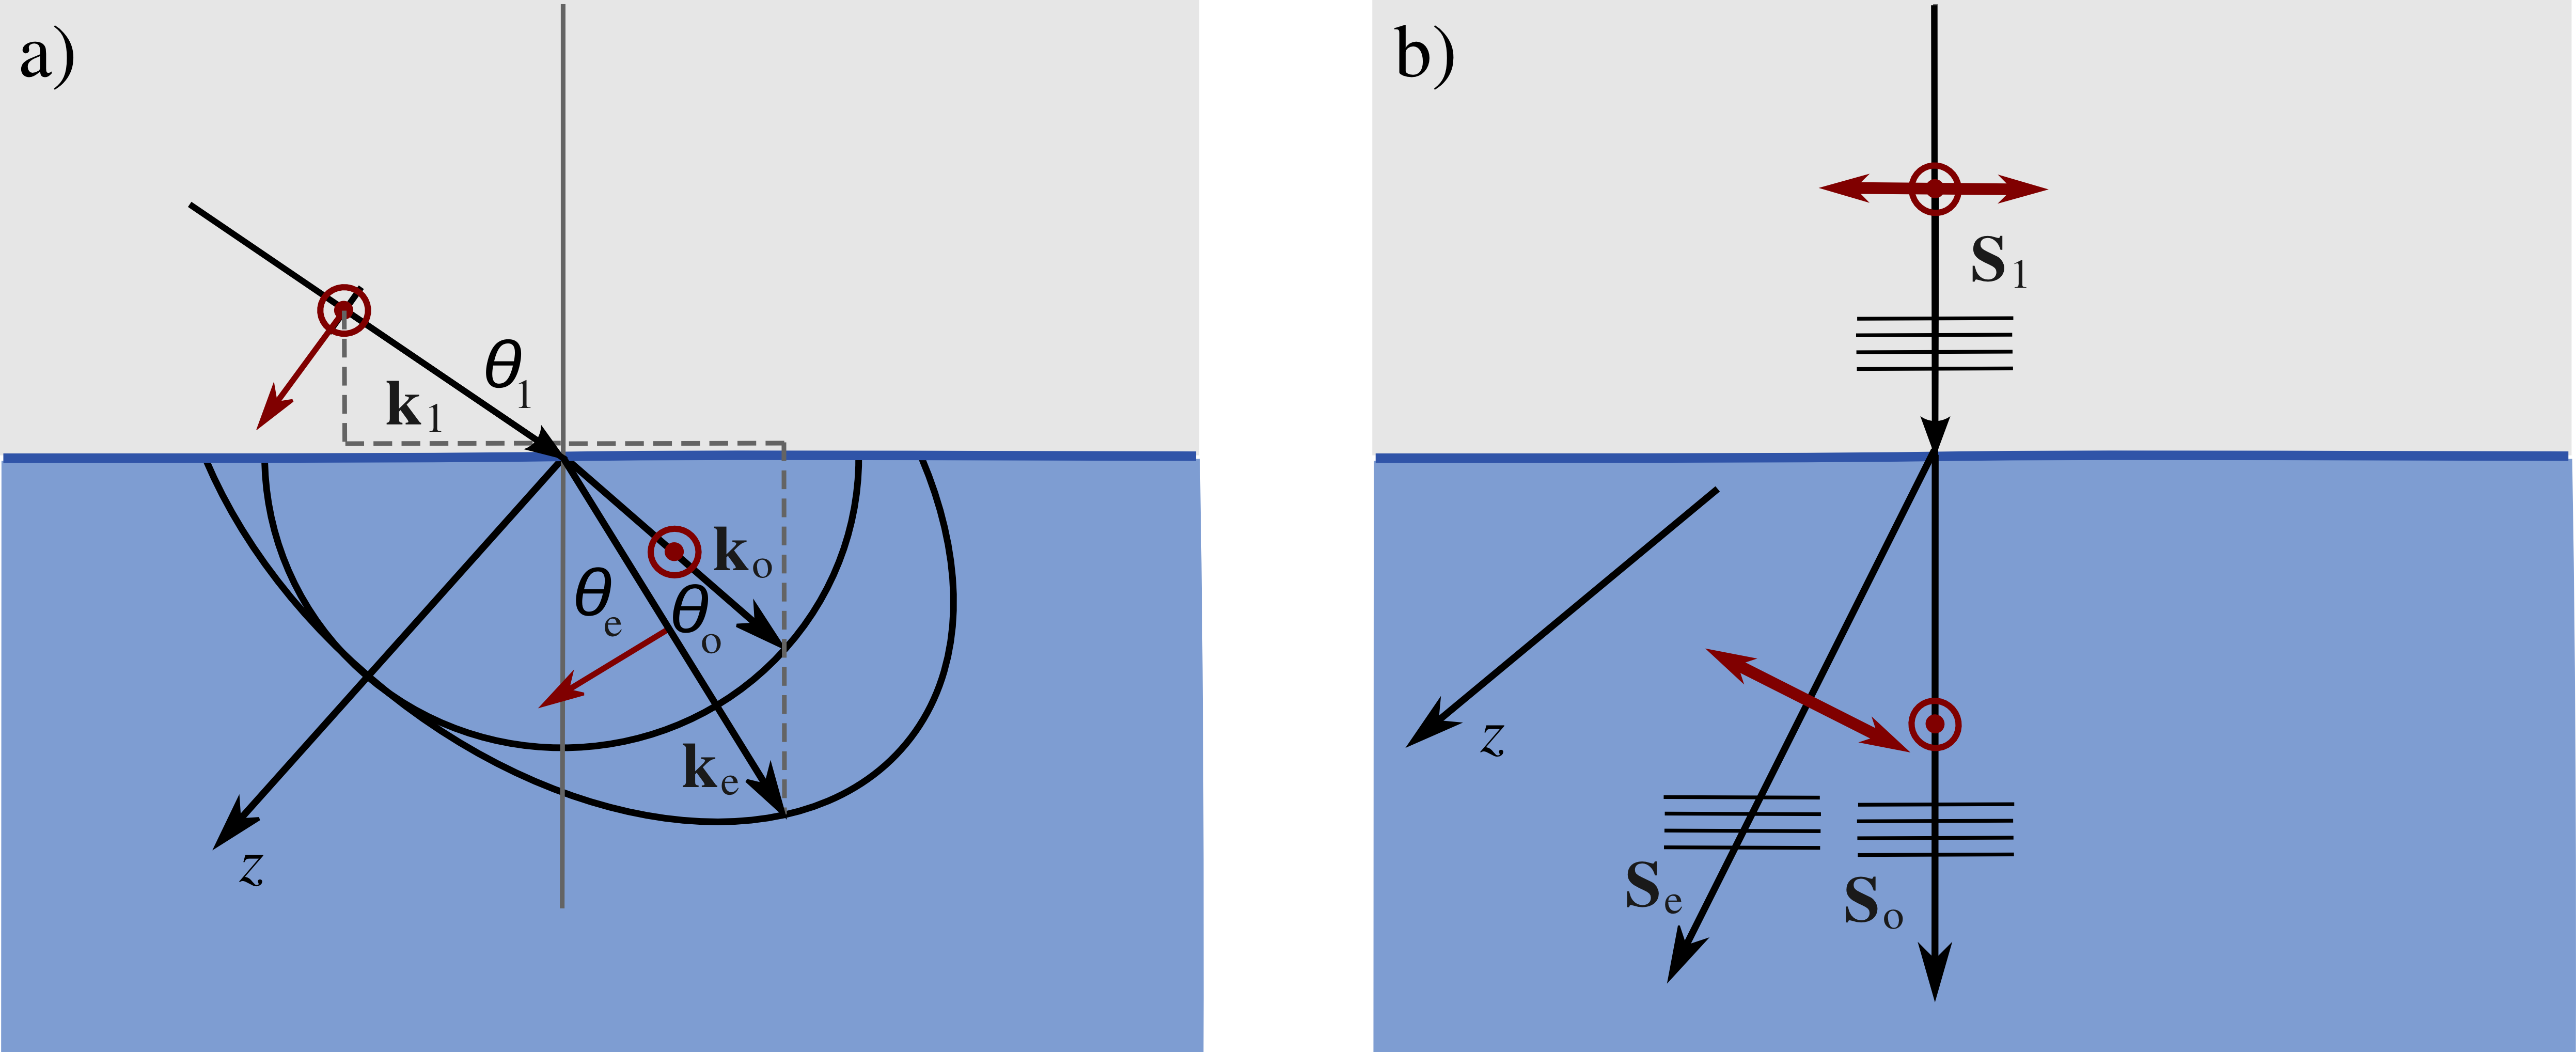
\includegraphics[width=12truecm]{slike/01_dvolom.png}
\caption{\label{fig:dvolomnost}Dvojni lom. a) Pri poševnem vpadu na anizotropno snov se
valovanje loči na dva različno polarizirana žarka. b) Tudi pri pravokotnem vpadu se žarka 
ločita, če je optična os pod poljubnim kotom glede na normalo mejne ravnine. Valovni vektorji
so v tem kolinearni, Poyntingovi vektorji pa imajo različne smeri.}
\end{figure}


Kadar vpada valovanje pravokotno na izotropno snov, se žarek ne lomi. V 
dvolomnih snoveh pa lahko tudi pri pravokotnem vpadu pride do razklona žarkov (slika
\ref{fig:dvolomnost}b). Kadar je optična os nagnjena glede na vpadnico, sta valovna vektorja
obeh prepuščenih žarkov sicer vzporedna valovnemu vektorju vpadnega žarka ($\mathbf{k}_1 \parallel
\mathbf{k}_o \parallel \mathbf{k}_e$), razlikujejo pa se smeri Poyntingovih vektorjev
($\mathbf{S}_1 \parallel \mathbf{S}_o \nparallel \mathbf{S}_e$). Ob prehodu skozi 
plast anizotropne snovi tako dobimo dva vzporedna, a razmaknjena žarka z medsebojno
pravokotnimi polarizacijami. Enoosne kristale, odrezane pod primernim kotom in prave dolžine,
zato lahko uporabimo kot polarizacijski delilnik žarkov.

